\subsection{Rozdzielenie wektorów na paczki}
Jednym ze sposobów przyspieszenia czasu uczenia jest podzielenie danych na paczki (ang. batche).
Pozwala nam to na wykonywanie obliczeń na wielu danych jednocześnie. W naszej bibliotece 
wymiarami batcha zawsze będzie: (rozmiar batcha) $\times$ (rozmiar alfabetu) $\times$ (liczba kroków czasowych). 
Poniżej przedstawiamy batchowanie na przykładzie, dla którego przyjmiemy następujące założenia: 
\begin{itemize}
	\item rozmiar batcha równy 3
	\item liczba kroków czasowych równa 3
	\item liczba autorów równa 4
	\item alfabet $\{a,b,c,d\}$
\end{itemize}

Każdy z autorów ma przyporządkowane nastpujące teksty:
\begin{itemize}
	\item autor 1: ``abacd''
	\item autor 2: ``dbaa''
	\item autor 3: ``cadb''
	\item autor 4: ``cbbcc''
\end{itemize}

Zamieniamy litery na wektory wedle wcześniejszego opisu, gdzie:
\vspace{3mm}
\newline 
$
a =
\begin{bmatrix} 
1, & 0, & 0, & 0
\end{bmatrix} 
$
\vspace{3mm}
\newline
$
b = 
\begin{bmatrix} 
0, & 1, & 0, & 0
\end{bmatrix} 
$
\vspace{3mm}
\newline 
$
c =
\begin{bmatrix} 
0, & 0, & 1, & 0
\end{bmatrix} 
$
\vspace{3mm}
\newline 
$
d =
\begin{bmatrix} 
0, & 0, & 0, & 1
\end{bmatrix} 
$
\vspace{1mm}
\newline 

Wektory umieszczamy w wektorach. Dla każdego autora przewidziany jest osobny wektor. 
Przykładowo dla autora 3 wyglądałby on następująco:
\vspace{3mm}

$
\begin{bmatrix} \begin{bmatrix} 0, & 0, & 1, & 0\end{bmatrix},  & \begin{bmatrix} 1, & 0, & 0, & 0\end{bmatrix}, & \begin{bmatrix} 0, & 0, & 0, & 1\end{bmatrix}, & \begin{bmatrix} 0, & 1, & 0, & 0\end{bmatrix} \end{bmatrix}
$



\begin{wrapfigure}{r}{0.6\textwidth}
\vspace{-4mm}
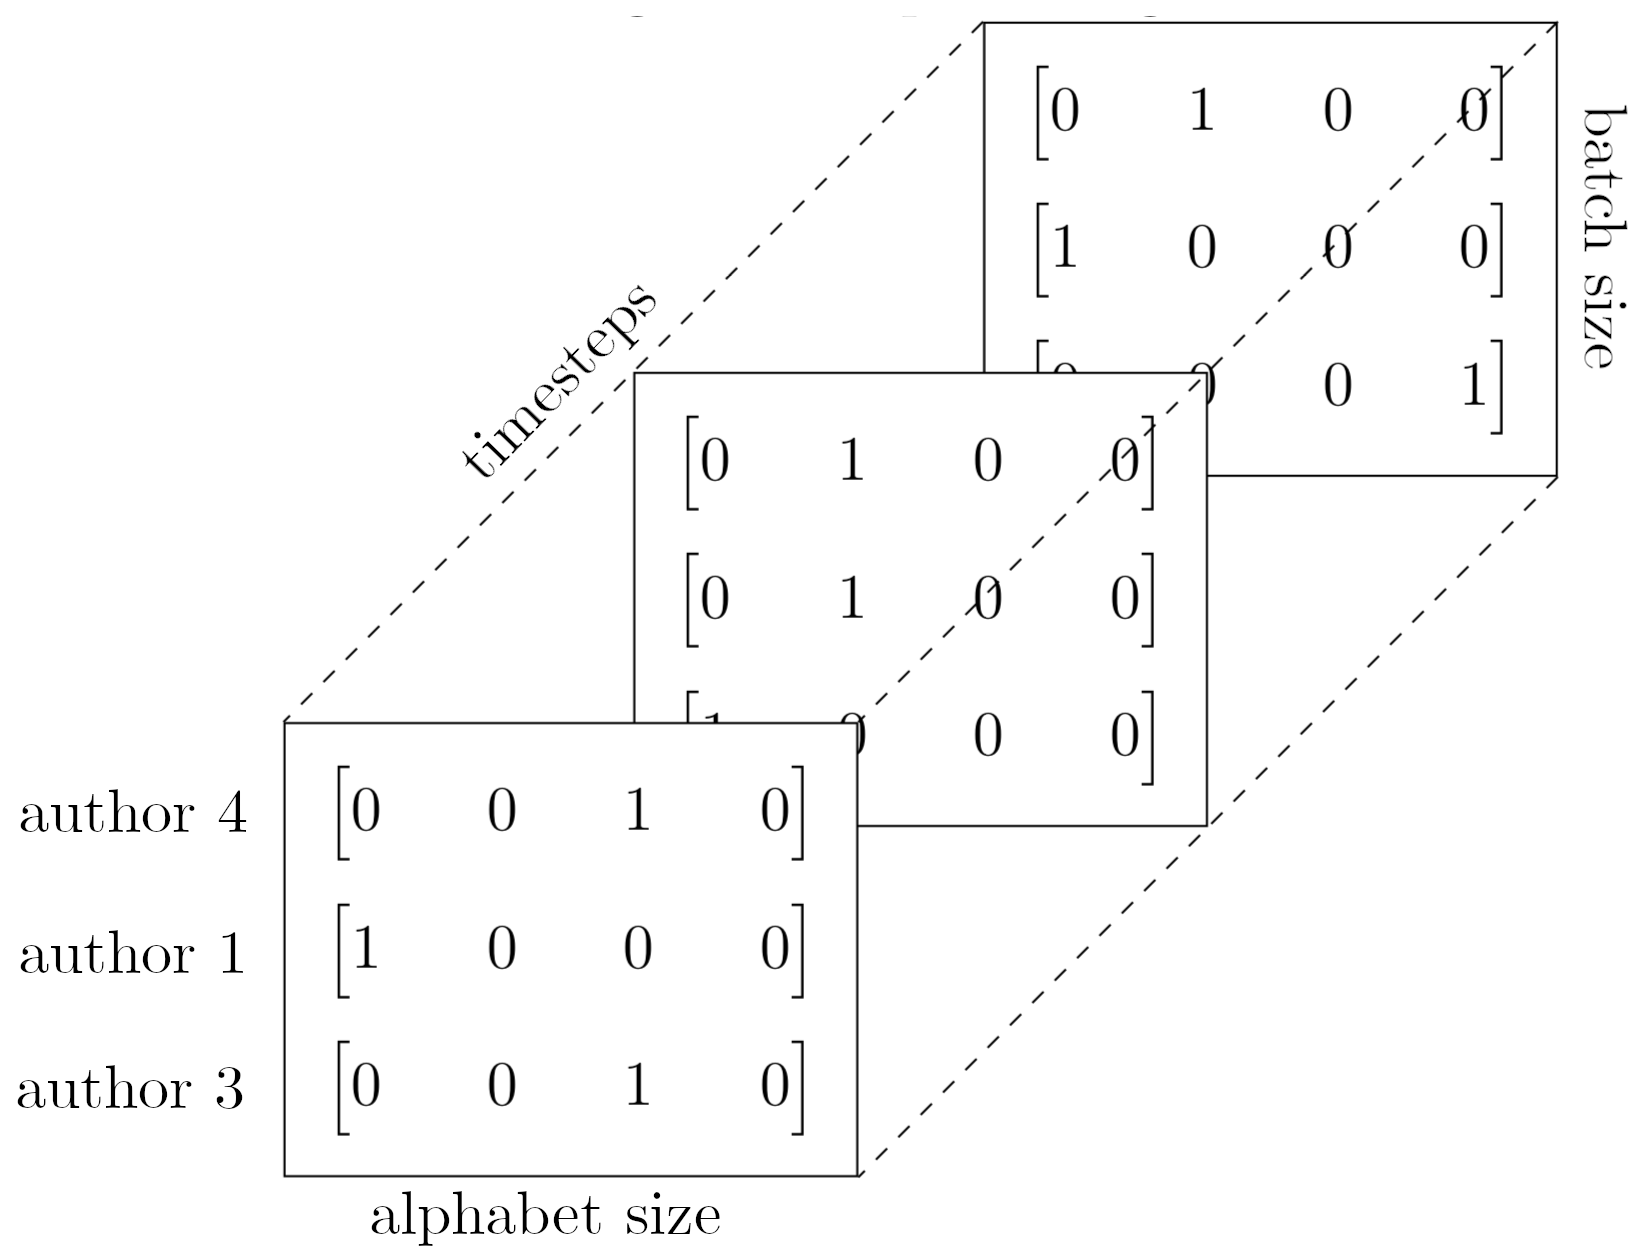
\includegraphics[width=\linewidth]{./images/batch.png}
\caption{Wizualizacja pierwszego batcha}
\label{fig:test2}
\vspace{-4mm}
\end{wrapfigure}
\vspace{4mm}
Następnie ze wszystkich tych wektorów tworzymy batche.
Dla tego przykładu każdy z batchy będzie wektorem o wymiarach $3 \times 4 \times 3$.
Do każdej takiej paczki będziemy losować autorów oraz ich kolejność. Załóżmy, że do pierwszego batcha
wylosowaliśmy autora 4, 1 oraz 3. Oznacza to, że w pierwszym kroku czasowym w wektorze zawarta będzie 
patrząc ``od góry'': pierwsza litera tekstu autora 4, pierwsza litera tekstu autora 1 oraz pierwsza litera tekstu autora 3.
To ustawienie autorów w wektorach będzie już zawsze zachowane dla wszystkich kroków czasowych w tym batchu. 
A więc dla drugiego kroku czasowego będzie to: druga litera tekstu autora 4, druga litera tekstu autora 1 oraz druga 
litera tekstu autora 3. Dla trzeciego kroku czasowego analogicznie. 

Może się zdarzyć sytuacja, że do batcha wylosowano kilkukrotnie tego samego autora. Na przykład wylosowano
autorów 1 oraz 3, w kolejności: autor pierwszy, następnie znowu autor pierwszy, na końcu autor trzeci.
Dla identycznych założeń jak we wcześniejszym przykładzie w pierwszym batchu w pierwszym kroku czasowym wyglądałoby to
 następująco: pierwsza litera tekstu autora 1, następnie pierwsza litera tekstu autora 1,
na końcu pierwsza litera tekstu autora 3. W drugim kroku czasowym byłoby to:
druga litera tekstu autora 1, druga litera tekstu autora 1 oraz druga litera tekstu autora 3, itd.

Liczba batchy jest zależna od długości tekstów. Są tworzone dopóki nie skończą się znaki w wektorze
najdłuższego tekstu jednego z autorów, dlatego teksty powinny być mniej więcej tej samej długości. Dopóki nie skończy się 
najdłuższy tekst, teksty krótsze są zapętlane i ponownie podawane do sieci.  Sieć można
wyszkolić dobrze tylko zachowując maksymalnie dużą losowość wystąpień autorów w każdym batchu.
